\documentclass{beamer}
\usetheme{Madrid}
\usefonttheme{professionalfonts}
\setbeamertemplate{navigation symbols}{}
\setbeamertemplate{footline}[frame number]

\usepackage{graphicx}
\usepackage{booktabs}
\usepackage{array}
\usepackage{tikz}
\usetikzlibrary{arrows.meta,positioning}

\newcommand{\safeimage}[2][]{%
  \IfFileExists{#2}{\includegraphics[#1]{#2}}{%
    \fbox{\parbox[c][0.25\textheight][c]{0.75\linewidth}{\centering Missing image:\\\texttt{#2}}}%
  }%
}

\title{Multifidus Muscle Classification from Ultrasound Imaging Using Deep Learning}
\author{Rahul Bisht \\ M241114CS \\ Guided by: Dr. Jayaraj PB}
\date{\today}

\begin{document}

\begin{frame}
\titlepage
\end{frame}

\begin{frame}
\frametitle{Presentation Flow}
\begin{itemize}
    \item Introduction, motivation, and problem statement
    \item Location of the lumbar multifidus muscle
    \item Paper reviews
    \item Dataset and class distribution
    \item Segmentation work and ROI crop
    \item Methodology and methodology images
    \item Binary classification results
    \item Previous Heckmatt grading results
    \item New work: direct classification, pairwise, hierarchy, audit, and UI tools
    \item Discussion, conclusion, and references
\end{itemize}
\end{frame}

%------------------------------------------------------------
\section{Introduction}

\begin{frame}
\frametitle{Introduction: Low Back Pain and Lumbar Multifidus}
\begin{itemize}
\item Low Back Pain (LBP) is one of the common musculoskeletal problems seen in daily life.
\item The Lumbar Multifidus Muscle (LMM) is a deep spinal muscle that supports segmental stability of the lower back.
\item LMM atrophy and fatty infiltration are strongly linked with chronic low back pain.
\item MRI and CT can be used for assessment, but they are costly or less suitable for repeated screening.
\item Ultrasound is safer and cheaper, but the image interpretation depends heavily on the observer.
\end{itemize}
\end{frame}

\begin{frame}
\frametitle{Motivation}
\begin{itemize}
\item \textbf{Clinical need:} Better LMM assessment can help in diagnosis and follow-up of low back pain.
\item CT exposes patients to ionizing radiation.
\item MRI is expensive and not suitable for all patients.
\item USG is safe, inexpensive, real-time, and widely accessible.
\item Manual USG grading has high inter-observer variability.
\item The goal is to build a deep learning based system that can support repeatable and objective assessment.
\end{itemize}
\end{frame}

\begin{frame}
\frametitle{Problem Statement}
\begin{itemize}
\item Given a B-mode ultrasound image of the lumbar multifidus region, the system should:
\begin{itemize}
    \item locate the muscle region,
    \item crop the region of interest,
    \item classify the image into Heckmatt grade H1, H2, H3, or H4.
\end{itemize}
\item The model should learn from echo intensity and texture changes.
\item The project also checks whether some class labels are inconsistent and need expert correction.
\end{itemize}
\end{frame}

\begin{frame}
\frametitle{Location of the Multifidus Muscle}
\begin{center}
\safeimage[width=0.82\textwidth,height=0.72\textheight,keepaspectratio]{muscle.png}
\end{center}
\end{frame}

\begin{frame}
\frametitle{Multifidus in Ultrasound}
\begin{center}
\safeimage[width=0.6\textwidth]{bmode.png}

\end{center}
\end{frame}

%------------------------------------------------------------
\section{Paper Reviews}

\begin{frame}
\frametitle{Paper Review: LMM and Low Back Pain}
\begin{itemize}
\item Freeman et al. studied the role of lumbar multifidus in chronic low back pain.
\item LMM dysfunction includes atrophy, fatty infiltration, and reduced stabilizing function.
\item MRI and ultrasound were discussed as useful tools for muscle assessment.
\item This supports the clinical motivation for automated LMM ultrasound analysis.
\end{itemize}
\end{frame}

\begin{frame}
\frametitle{Paper Review: DL Challenges in Muscle USG}
\begin{itemize}
\item Ardhianto et al. reviewed challenges in deep learning for skeletal and smooth muscle ultrasound images.
\item Key issues:
\begin{itemize}
    \item low image quality,
    \item motion artifacts,
    \item speckle noise,
    \item limited annotated data.
\end{itemize}
\item The review supports the need for preprocessing, cropping, and careful dataset handling.
\end{itemize}
\end{frame}

\begin{frame}
\frametitle{Paper Review: LMM Thickness and Fat Quantification}
\begin{itemize}
\item Kim et al. proposed an automated system for LMM thickness and intramuscular fat estimation from ultrasound.
\item Contrast enhancement was used to improve muscle boundary visibility.
\item Fuzzy C-Means clustering was used for fat-related pixel grouping.
\item The work shows that ultrasound texture and intensity can carry useful muscle-quality information.
\end{itemize}
\end{frame}

\begin{frame}
\frametitle{Paper Review: LUMINOUS Dataset}
\begin{itemize}
\item Belasso et al. introduced the LUMINOUS database for lumbar multifidus ultrasound segmentation.
\item It contains B-mode ultrasound images and manually segmented masks.
\item The dataset was collected from young athletic adults.
\item In this project, LUMINOUS masks were used to derive bounding boxes for ROI detection.
\item Limitation: the population is different from clinical GMC data, so domain shift is expected.
\end{itemize}
\end{frame}

\begin{frame}
\frametitle{Paper Review: Other Medical Imaging Work}
\begin{itemize}
\item Weber et al. used CNNs for cervical muscle segmentation and muscle fat infiltration estimation.
\item Rodriguez et al. showed that preprocessing affects ultrasound segmentation and classification.
\item CACTUS showed that large ultrasound datasets can improve transfer learning performance.
\item Kidney stone detection studies show that ML/DL can work well on ultrasound when data and preprocessing are handled properly.
\end{itemize}
\end{frame}

%------------------------------------------------------------
\section{Dataset}

\begin{frame}
\frametitle{Datasets Used}
\begin{itemize}
\item \textbf{LUMINOUS dataset}
\begin{itemize}
    \item public lumbar multifidus ultrasound dataset,
    \item includes manually segmented masks,
    \item used mainly for segmentation and ROI detection experiments.
\end{itemize}
\item \textbf{GMC / project dataset}
\begin{itemize}
    \item clinical ultrasound images,
    \item labelled into Heckmatt grades,
    \item used for classification, pairwise, hierarchy, and audit experiments.
\end{itemize}
\item Recent experimental phase used \textbf{606 labelled images}.
\end{itemize}
\end{frame}

\begin{frame}
\frametitle{Dataset Distribution}
\begin{center}
\safeimage[width=0.82\textwidth,height=0.70\textheight,keepaspectratio]{datasetDistribution.png}
\end{center}
\end{frame}

\begin{frame}
\frametitle{Dataset Imbalance}
\begin{itemize}
\item Class distribution:
\begin{itemize}
    \item H1: 146 images
    \item H2: 279 images
    \item H3: 129 images
    \item H4: 52 images
\end{itemize}
\item H2 is the dominant class.
\item H4 has the fewest images.
\item Since the classes are imbalanced, accuracy alone is not enough.
\item Balanced accuracy and confusion matrices were used for better interpretation.
\end{itemize}
\end{frame}

%------------------------------------------------------------
\section{Segmentation and ROI}

\begin{frame}
\frametitle{Segmentation Work}
\begin{itemize}
\item U-Net with ResNet-34 encoder was trained for LMM segmentation.
\item LUMINOUS masks and annotated GMC images were used.
\item Images were resized to 256 $\times$ 256.
\item Results on LUMINOUS:
\begin{itemize}
    \item IoU = 0.86
    \item Dice = 0.92
    \item Pixel Accuracy = 0.98
\end{itemize}
\item Performance dropped on GMC images because of domain shift.
\end{itemize}
\end{frame}

\begin{frame}
\frametitle{Segmentation Output}
\begin{center}
\safeimage[width=0.28\textwidth]{bmode.png}
\hspace{0.4cm}
\safeimage[width=0.28\textwidth]{groundtruthmask.png}
\hspace{0.4cm}
\safeimage[width=0.28\textwidth]{predicted mask.png}

\vspace{0.25cm}
\small B-mode Image \hspace{1.3cm} Ground Truth \hspace{1.2cm} Predicted Mask
\end{center}
\end{frame}

\begin{frame}
\frametitle{Image Segmentation and Crop}
\begin{center}
\safeimage[width=0.36\textwidth]{11.3 (1).jpg}
\hspace{0.8cm}
\safeimage[width=0.36\textwidth]{roi_cut.jpg}

\vspace{0.3cm}
\small Original ultrasound image \hspace{1.5cm} Cropped ROI
\end{center}
\begin{itemize}
\item The final classifier works on the focused LMM region.
\item Cropping reduces irrelevant background information.
\end{itemize}
\end{frame}

\begin{frame}
\frametitle{ROI Extraction: Model Progression}
\begin{itemize}
\item \textbf{U-Net:} good segmentation on LUMINOUS, weaker generalization to GMC.
\item \textbf{SAM:} strong when bounding-box prompt is provided, but prompt requirement is impractical.
\item \textbf{YOLOv8m:} selected because it predicts bounding boxes directly.
\item YOLOv8m validation results:
\begin{itemize}
    \item mAP50 = 0.995
    \item Precision = 0.999
    \item Recall = 1.0
\end{itemize}
\end{itemize}
\end{frame}

%------------------------------------------------------------
\section{Methodology}



\begin{frame}
\frametitle{Methodology Image: YOLO Fine-Tuning}
\begin{center}
\safeimage[width=0.95\textwidth,height=0.76\textheight,keepaspectratio]{Screenshot 2026-02-25 232024.png}
\end{center}
\end{frame}

\begin{frame}
\frametitle{Methodology Image: YOLO Architecture}
\begin{center}
\safeimage[width=0.90\textwidth,height=0.72\textheight,keepaspectratio]{Architecture-of-the-YOLO-network.png}
\end{center}
\end{frame}

\begin{frame}
\frametitle{Methodology Image: Classification Pipeline}
\begin{center}
\safeimage[width=0.78\textwidth,height=0.72\textheight,keepaspectratio]{yolo_arch.png}
\end{center}
\end{frame}

\begin{frame}
\frametitle{Methodology Image: EfficientNet Architecture}
\begin{center}
\safeimage[width=0.80\textwidth,height=0.72\textheight,keepaspectratio]{EfficientNet-Architecture.png}
\end{center}
\end{frame}

\begin{frame}
\frametitle{Methodology Image: Hierarchical Inference}
\begin{center}
\safeimage[width=0.95\textwidth,height=0.76\textheight,keepaspectratio]{hierarchical-inf-pipe.png}
\end{center}
\end{frame}

\begin{frame}
\frametitle{Methodology Image: Label Audit}
\begin{center}
\safeimage[width=0.95\textwidth,height=0.76\textheight,keepaspectratio]{label-audit.png}
\end{center}
\end{frame}

%------------------------------------------------------------
\section{Binary Classification}

\begin{frame}
\frametitle{Binary Classification: Normal vs Abnormal}
\begin{itemize}
\item Earlier experiments grouped images into normal and abnormal classes.
\item Three pretrained backbones were evaluated with a classification head.
\item Results:
\begin{itemize}
    \item EfficientNet-B0: 90.47\% accuracy
    \item ViT-B16: 90.47\% accuracy
    \item SigLIP encoder: 85.71\% accuracy
\end{itemize}
\item Binary classification was easier than four-class Heckmatt grading.
\end{itemize}
\end{frame}

\begin{frame}
\frametitle{Binary Classification: ViT-B16}
\begin{itemize}
\item Accuracy: 90.47\%
\item Precision: 0.9412
\item Recall: 0.9412
\item F1-score: 0.9412
\end{itemize}
\begin{center}
\safeimage[width=0.35\textwidth]{confusion_matrix.png}
\end{center}
\end{frame}



%------------------------------------------------------------
\section{Previous Heckmatt Work}

\begin{frame}
\frametitle{Previous Heckmatt Grading Work}
\begin{itemize}
\item The binary task was extended to four Heckmatt grades.
\item Earlier runs tested different pretrained backbones.
\item The initial four-class results were weaker than binary classification.
\item Main difficulty: adjacent grades looked visually similar and the class distribution was imbalanced.
\end{itemize}
\end{frame}

\begin{frame}
\frametitle{Previous Heckmatt Results}
\begin{center}
\begin{tabular}{lcc}
\toprule
\textbf{Model} & \textbf{Best Val Acc.} & \textbf{Test Acc.}\\
\midrule
ViT-B16 cropped & 64.00\% & 47.00\%\\
MedGemma vision & 62.00\% & 50.00\%\\
ViT-B16 full image & 61.11\% & 55.00\%\\
ResNet & 53.30\% & 51.10\%\\
EfficientNet-B0 & 52.00\% & 50.00\%\\
\bottomrule
\end{tabular}
\end{center}
\begin{itemize}
\item ViT full-image model gave the best earlier test accuracy.
\item MedGemma did not clearly improve performance in this dataset.
\end{itemize}
\end{frame}

\begin{frame}
\frametitle{Previous Heckmatt Confusion Example}
\begin{center}
\safeimage[width=0.55\textwidth,height=0.66\textheight,keepaspectratio]{MedGemmaconfusionmatrix.png}
\end{center}
\end{frame}

%------------------------------------------------------------
\section{New Work}

\begin{frame}
\frametitle{New Work Added in This Phase}
\begin{itemize}
\item Direct four-class classification with updated baselines and gaussian blur.
\item ViT hyperparameter search.
\item Pairwise binary classifiers for every Heckmatt pair.
\item Hierarchical inference in both directions.
\item Binary label audit using normal/abnormal grouping.
\item Annotation tool for doctor-led label correction.
\end{itemize}
\end{frame}

\begin{frame}
\frametitle{Direct Four-Class Classification}
\begin{center}
\begin{tabular}{lcc}
\toprule
\textbf{Experiment} & \textbf{Test Accuracy} & \textbf{Test Loss}\\
\midrule
Equalized ViT & 50.55\% & 2.4477\\
ViT + augmentation & 60.20\% & --\\
ViT + Gaussian blur & 57.14\% & 2.102\\
ResNet18 direct & 63.74\% & 1.6417\\
\bottomrule
\end{tabular}
\end{center}
\begin{itemize}
\item ResNet18 gave the strongest direct four-class result.
\item H4 was handled well despite having fewer samples.
\end{itemize}
\end{frame}

\begin{frame}
\frametitle{Direct ResNet18 Confusion Matrix}

\begin{center}
\safeimage[width=0.58\textwidth]{confusion\_matrix\_resnet.png}
\end{center}


\begin{itemize}
\item Main confusion: H1/H2 and H2/H3.
\item H4 remains the cleanest class.
\end{itemize}
\end{frame}

\begin{frame}
\frametitle{Hyperparameter Search}
\begin{itemize}
\item 36 ViT runs were performed.
\item Search dimensions:
\begin{itemize}
    \item learning rate,
    \item dropout,
    \item batch size,
    \item number of unfrozen final blocks.
\end{itemize}
\item Trial 32 had best validation accuracy.
\item Trials 15 and 19 gave better test accuracy and balanced accuracy.
\item Validation loss and validation accuracy did not always move in the same direction.
\end{itemize}
\end{frame}

\begin{frame}
\frametitle{Hyperparameter Search Results}
\begin{center}
\begin{tabular}{lccccc}
\toprule
\textbf{Trial} & \textbf{LR} & \textbf{Dropout} & \textbf{Batch} & \textbf{Test Acc.} \\
\midrule
15 & 0.0003 & 0.2 & 8 & 61.50\% \\
19 & 0.0003 & 0.3 & 8 & 61.50\% \\
29 & 0.0010 & 0.3 & 8 & 60.40\% \\
25 & 0.0010 & 0.2 & 8 & 60.40\% \\
32 & 0.0010 & 0.3 & 16 & 54.90\% \\
\bottomrule
\end{tabular}
\end{center}
\end{frame}

\begin{frame}
\frametitle{Pairwise Binary Experiments}
\begin{itemize}
\item Pairwise models were trained to check grade-boundary separability.
\item Distant grades were easier to separate.
\item Middle grade boundaries were weaker.
\end{itemize}
\begin{center}
% \begin{tabular}{lcc}
% \toprule
% \textbf{Pair} & \textbf{Accuracy} & \textbf{Balanced Accuracy}\\
% \midrule
% H1 vs H2 & 70.45\% & 70.45\%\\
% H1 vs H3 & 84.21\% & 84.21\%\\
% H1 vs H4 & 93.75\% & 93.70\%\\
% H2 vs H3 & 60.53\% & 60.53\%\\
% H2 vs H4 & 93.75\% & 93.70\%\\
% H3 vs H4 & 62.50\% & 62.50\%\\
% \bottomrule
% \end{tabular}


\safeimage[width=0.67\textwidth]{heatmap_pairwise.png}
\end{center}

\end{frame}

\begin{frame}
\frametitle{Pairwise Interpretation}
\begin{itemize}
\item H1 vs H4 and H2 vs H4 were the strongest pairs.
\item H2 vs H3 was the weakest pair.
\item This suggests the middle Heckmatt boundaries are not very clear.
\item Pairwise results support the label-audit finding that some samples need review.
\end{itemize}
\end{frame}

\begin{frame}
\frametitle{Hierarchical Inference Results}
\begin{center}
\begin{tabular}{lccccc}
\toprule
\textbf{Cascade} & \textbf{Acc.} & \textbf{H1} & \textbf{H2} & \textbf{H3} & \textbf{H4}\\
\midrule
EfficientNet low-high & 52.75\% & 13.6\% & 73.8\% & 42.1\% & 75.0\%\\
ResNet18 low-high & 53.85\% & 54.5\% & 57.1\% & 26.3\% & 100.0\%\\
ResNet18 high-low & 61.54\% & 50.0\% & 71.4\% & 36.8\% & 100.0\%\\
\bottomrule
\end{tabular}
\end{center}
\begin{itemize}
\item High-to-low ResNet18 performed best.
\item H4 recall remained perfect in ResNet18 cascades.
\item Middle-grade decisions were still unstable.
\end{itemize}
\end{frame}

\begin{frame}
\frametitle{Label Audit Setup}
\begin{itemize}
\item H1 and H2 were treated as normal.
\item H3 and H4 were treated as abnormal.
\item ViT binary predictions were compared with this assumed grouping.
\item Disagreement means the predicted binary label did not match the assumed binary label.
\item High-confidence disagreement threshold: confidence $\geq 0.8$.
\end{itemize}
\end{frame}

\begin{frame}
\frametitle{Label Audit Results}
\begin{center}
\begin{tabular}{lc}
\toprule
\textbf{Metric} & \textbf{Value}\\
\midrule
Total images & 606\\
Disagreements & 172\\
Disagreement rate & 28.38\%\\
High-confidence disagreements & 79\\
High-confidence disagreement rate & 13.04\%\\
\bottomrule
\end{tabular}
\end{center}
\end{frame}

\begin{frame}
\frametitle{Label Audit: Class-wise Findings}
\begin{center}
\scriptsize
\begin{tabular}{lccccc}
\toprule
\textbf{Class} & \textbf{Assumed} & \textbf{Total} & \textbf{Agree} & \textbf{Disagree} & \textbf{High-conf.}\\
\midrule
H1 & Normal & 146 & 120 & 26 & 6\\
H2 & Normal & 279 & 203 & 76 & 41\\
H3 & Abnormal & 129 & 68 & 61 & 29\\
H4 & Abnormal & 52 & 43 & 9 & 3\\
\bottomrule
\end{tabular}
\end{center}
\begin{itemize}
\item H2 had the largest number of disagreements: 76 out of 279 images.
\item H3 had the highest disagreement rate: 61 out of 129 images.
\item H2 and H3 also produced most high-confidence disagreements.
\item This supports the need for doctor-led label correction.
\end{itemize}
\end{frame}

\begin{frame}
\frametitle{Clinical User Interface}
\begin{itemize}
\item Upload ultrasound images.
\item Display YOLO-detected ROI.
\item Show predicted Heckmatt grade.
\item Designed for physicians and non-technical users.
\end{itemize}
\begin{center}
\safeimage[width=0.58\textwidth,height=0.42\textheight,keepaspectratio]{UI.jpg}
\end{center}
\end{frame}

\begin{frame}
\frametitle{Annotation Tool for Label Correction}
\begin{itemize}

\item Images are shown to the clinician one by one.
\item The doctor can create bounding boxes around muscle.
\item The doctor can label the unlabeled images.
\item This was further extended to relabel the images for label correction.
\item Corrected labels and bounding boxes can be downloaded using a button.
\end{itemize}
\end{frame}

\section{Annotation Screenshot}
\begin{frame}
\begin{center}
\safeimage[width=0.9\textwidth]{annotation.png}
\end{center}
\end{frame}

%------------------------------------------------------------
\section{Discussion and Conclusion}

\begin{frame}
\frametitle{Results and Discussion}
\begin{itemize}
\item Binary classification performed strongly, but four-class grading was harder.
\item Pairwise and hierarchical experiments showed unclear middle-grade boundaries.
\item H4 performed well even with fewer samples, so the problem is not only data quantity.
\item The audit showed that label correction is a key part of the next phase.
\item On merging class 3-4 accuracy jumped to 62\% from 50\% on efficient net.
\item On merging class 2-3 74.71\% accuracy was achieved.
\end{itemize}
\end{frame}

\begin{frame}
\frametitle{Training Curve Observation}
\begin{itemize}
\item In several experiments, validation accuracy improved while validation loss increased.
\item Test loss did not always follow the same direction.
\item This suggests that some predictions became more confident even when labels or boundaries were uncertain.
\item This supports the decision to perform label audit and doctor review.
\end{itemize}
\end{frame}

\begin{frame}{Loss and accuracy plot}

\begin{figure}[h]
    \centering
        \begin{minipage}{0.48\textwidth}
        \centering
        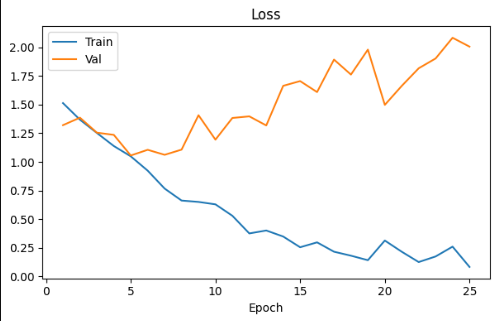
\includegraphics[width=\linewidth]{loss.png}
        \caption{Loss plot}
    \end{minipage}
    % Left image
    \begin{minipage}{0.48\textwidth}
        \centering
        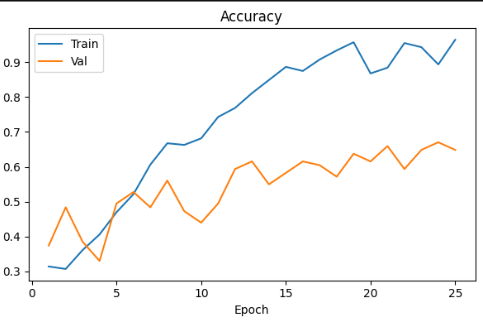
\includegraphics[width=\linewidth]{accuracy.png}
        \caption{Accuracy plot}
    \end{minipage}
    \hfill
    % Right image

    
\end{figure}

\end{frame}

\begin{frame}
\frametitle{Conclusion}
\begin{itemize}
\item An automated LMM ultrasound workflow was developed.
\item The system includes ROI extraction, classification, audit, and annotation support.
\item YOLOv8 was selected for ROI detection.
\item ResNet18 gave the best direct four-class result.
\item Pairwise and hierarchy logs showed that H2/H3 and H3/H4 are weak boundaries.
\item Label audit identified cases that should be reviewed first.
\end{itemize}
\end{frame}

\begin{frame}
\frametitle{Future Work}
\begin{itemize}
\item Complete doctor-led correction of uncertain labels.
\item Retrain all models on corrected labels.
\item Add more data, especially for H3 and H4.
\item Improve domain adaptation between LUMINOUS and GMC images.
\item Test ultrasound foundation models such as USFM and UltraSam.
\item Validate the system against expert clinical grading.
\end{itemize}
\end{frame}

%------------------------------------------------------------
\section{References}

\begin{frame}
\frametitle{References}
\begin{itemize}
\item [1] Freeman, M.D.; Woodham, M.A.; Woodham, A.W. The role of the lumbar multifidus in chronic low back pain: A review. PM\&R, 2010.
\item [2] Ardhianto, P. et al. A Review of the Challenges in Deep Learning for Skeletal and Smooth Muscle Ultrasound Images. Applied Sciences, 2021.
\item [3] Kim, K.B.; Park, H.J.; Song, D.H. Automatic characterizations of lumbar multifidus muscle and intramuscular fat from ultrasound images. Current Medical Imaging, 2020.
\end{itemize}
\end{frame}

\begin{frame}
\frametitle{References}
\begin{itemize}
\item [4] Belasso, C.J. et al. LUMINOUS database: lumbar multifidus muscle segmentation from ultrasound images. BMC Musculoskeletal Disorders, 2020.
\item [5] Weber, K.A. et al. Multi-muscle deep learning segmentation to automate quantification of muscle fat infiltration. Scientific Reports, 2021.
\item [6] Rodriguez-Cristerna, A. et al. Impact of preprocessing approaches on breast ultrasound segmentation and classification. CCE, 2017.
\end{itemize}
\end{frame}

\begin{frame}
\frametitle{References}
\begin{itemize}
\item [7] Elmekki, H. et al. CACTUS: automated cardiac assessment and classification of ultrasound images using deep transfer learning. Computers in Biology and Medicine, 2025.
\item [8] Asaye, Y.A.; Annamalai, P.; Ayalew, L.G. Detection of kidney stone from ultrasound images using machine learning algorithms. Scientific African, 2025.
\item [9] Tan, M.; Le, Q. EfficientNet: Rethinking model scaling for convolutional neural networks. ICML, 2019.
\end{itemize}
\end{frame}

\end{document}
